\documentclass{resume} % Use the custom resume.cls style

\usepackage[left=0.75in,top=0.6in,right=0.75in,bottom=0.6in]{geometry} % Document margins
\usepackage{graphicx}
%\graphicspath{{images/}}
\name {Mohammed Ismail} % Your name
\address {S/O Mohammed Nissar 252 Fourth Cross Kote Area, Old Town Bhadravathi-577301}
\address{Shimoga(Dist.) Karnataka (S)} % Your address
\address{+919916235942 \\ mohammedismail.jnnce@gmail.com} % Your phone number and email

\begin{document}
\begin{figure}[h]

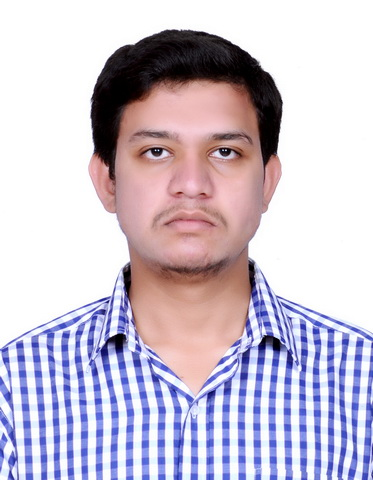
\includegraphics[height=4cm,width=3cm]{Ismail.jpg}\\
%\caption{Block Diagram of Remote Automation and Data monitoring of Irrigation System}\label{fig 2.1}
\end{figure}
\begin{rSection}{Career Objective}
To pursue an optimistic and challenging career in the field of IT Industry which gives me a scope to enhance my knowledge and skills in order to cope up with the latest technological changes
\end{rSection}

\begin{rSection}{Education}
\begin{center}
	\begin{tabular}{||c|c|c|c|c||}
		\hline\hline
		\bf Examination & \bf Institute & \bf University & \bf Year & \bf Performance \\
		\hline\hline
	    B.E(ECE) & JNN College of Engineering & VTU & 2015 & 75.21\% \\
		\hline
		II PUC/XII & SAV Composite PU College  & Karnataka State Board & 2011 & 91.16\% \\
		\hline
		SSLC/X & Sri Kanaka Vidya Samsthe  & Karnataka State Board & 2009 & 90.40\% \\
		\hline\hline
		
		
	\end{tabular}
\end{center}

\end{rSection}

\begin{rSection}{Projects}



\begin{enumerate}

\item \begin{rSubsection}{Weed Removal Robot}{December-2013}{e-yantra Robotics Competition-2014}{IIT-Bombay}
\item Role description: Designing of Robotic arm and identifying the weeds based on IR Sensor Values.
\end{rSubsection}

\item \begin{rSubsection}{Mobile based Voting Machine}{April, 2014}{Electronics \& Communication}{JNNCE,Shivamogga}
\item Purpose/Organization: Spectrum Project Exhibition-JNNCE
\item Role description: Interfacing MSP430 to GSM module, determine the polling status and display it on LCD.
\end{rSubsection}

\item \begin{rSubsection}{Fire Fighting Robot}{December, 2014}{e-yantra Robotics Competition-2015}{IIT-Bombay}
\item Role description: Designing of Fire-fighting Assembly and identifying the fire and extinguishing it based on conclusion derived from White Line Sensor Values.
\end{rSubsection}

\item \begin{rSubsection}{Remote Automation in Agriculture}{April, 2015}{Electronics \& Communication}{JNNCE,Shivamogga}
\item Automating a agricultural field by sending an SMS to the system which checks the various parameters such as availabilty of ground water,Soil moisture level,Three phase availability and whether its raining are not and then Switches on the MOTOR if all the parameters are satisfied.
\end{rSubsection}

\item \begin{rSubsection}{Workshops Conducted}{July, 2014}{Electronics \& Communication}{JNNCE,Shivamogga}
\item Conducted �Hobby Project Hands on Workshop� for 3rd Sem EC students.
\item Conducted �MSP 430 Microcontroller Hands on Workshop� for 5th Sem EC students of our college.
\end{rSubsection}

\end{enumerate}
\end{rSection}


\begin{rSection}{Training and Internship}
	\begin{itemize}
		%\item \begin{rSubsection}{Vocational Training on Telecom Technologies}{January, 2014}{Electronics \& Communication}{BSNL,Shivamogga}
         %   \item Successfully completed the communication training in BSNL.
			%\end{rSubsection}
		\item Successfully completed 3 days of Workshop on Basic Soldering and PCB Design Coarse conducted by Department of EC of our college.
        \item Attended 2 days Workshop on "Wireless Sensor Network and Robotics" organized by Kerala State Planning Board.
        \item Presently doing Internship at IIT BOMBAY,Mumbai on Robotics and Embedded C.
	\end{itemize}
\end{rSection}

\begin{rSection}{Research Publication}
	\begin{enumerate}
		\item Read a research paper on \textbf{Haptics Technology} as a part of an academic activity.
		\item Presented the Paper titled \textbf{Weed Removal Robot - a Firebird-V Overview} at the \textbf{National Technical Paper Contest-2014} held at KMEA College of Engineering Kerala. This Paper was awarded \textbf{First Prize} at the \textbf{57th IETE Student Session and Award Ceremony} held at IETE head quarter New Delhi.
        \item Presented the Paper titled Weed Removal Robot - a Firebird-V Overview  at \textbf{emanthana-2014} a National Level Paper Presentation Competition held at Adichinchinagiri Institute of Technology Chickmagalur and Secured \textbf{First Prize}.
	\end{enumerate}
\end{rSection}

\begin{rSection}{Technical Skills}
\begin{itemize}
		\item Coding and Debugging
		\item Programming and Problem Solving
		\item Testing and TroubleShooting
		\item Robotics
\end{itemize}
\end{rSection}

\begin{rSection}{Soft Skills}
	\begin{enumerate}
		\item C++, C, Embedded C, % Python
		\item Latex
		%\item Oscad
		\item Matlab
		
	\end{enumerate}
\end{rSection}
\begin{rSection}{Extra-Curricular Activities}
	\begin{itemize}
        \item Sanctioned Merit Scholarship from the MHRD, Govt. of India in II PUC.
        \item Participated in \textbf{e-yantra-2015} a National Level Robotics Challenge organised by IIT Bombay and grabbed 1st Place among 52 teams.
        \item Participated in World skills competition in the field of Mobile Robotics conducted by National skills Development Corporation.
        \item Selected for Texas instrument sponsored India Analog Competition-2015.
        \item Won first prize in National level Project Competition conducted by IETE at Amrutha College of Engineering,Coimbatore.
		\item Won Second Prize in Debate at
              Techzone 2K15,a National Level Technical Symposium held in our College.
        \item Participated in \textbf{e-yantra-2014} a National Level Robotics Challenge organised by IIT Bombay.
        \item Won first prize in National level Project Competition conducted by IETE at Amrutha College of Engineering,Coimbatore.
		\item Won Second Prize in Debate at
              Techzone 2K15,a National Level Technical Symposium held in our College.
	\end{itemize}
\end{rSection}

\begin{rSection}{Co-Curricular activities}
	\begin{enumerate}
    \item Served as a Coordinator at JNNCE's EC and TCE student's Technical forum called "Spectrum" for the year 2014.
    \item Served as the editor for ECE and TCE Students newsletter called "SAIL" for the year 2015.
    \item Served as a Volunteer at NSS-JNNCE
	\end{enumerate}
\end{rSection}

\begin{rSection}{Hobbies and Interest}
    \begin{itemize}
    \item Watching movies.
    \item Reading and Writing Essays.
    \item Playing Chess
    \end{itemize}
\end{rSection}
\begin{rSection}{Personal Information}
	\item \textbf{Father�s Name:} Mohammed Nissar
	\item \textbf{Mother�s Name: } Shamshul Huda
	\item \textbf{Gender:} Male
	\item \textbf{Date of Birth:} 8th January,1994
	\item \textbf{Nationality: } Indian
	\item \textbf{Marital Status:}	Single
\end{rSection}


\begin{rSection}{Declaration}
	I hereby declare that the above written particulars are true to the best of my knowledge and belief.
\end{rSection}
\begin{rSection}
	\bf \textbf{Date}
    %%\bf \textbf{Place}
\end{rSection}

 \end{document} 